\documentclass[12pt]{article}
%%% DOCUMENT FORMATTING %%%
\usepackage[margin=1in]{geometry}
\usepackage{enumitem}
\setlength{\parindent}{0pt}
\newcommand{\disp}{\displaystyle}

%%% HEADER %%%
\usepackage{fancyhdr}
\pagestyle{fancy}
\fancyhf{}
\lhead{MATH 1060}
\rhead{Vagnozzi}
\cfoot{\thepage}

%%% MATH NOTATION & SYMBOLS %%%
\usepackage{amssymb}
\usepackage{amsmath}
\newcommand{\R}{\mathbb{R}}
\newcommand{\N}{\mathbb{N}}
\newcommand{\Z}{\mathbb{Z}}
\newcommand{\lp}{\left(}
\newcommand{\rp}{\right)}
\newcommand{\ls}{\left[}
\newcommand{\rs}{\right]}
\newcommand{\lb}{\left\{}
\newcommand{\rb}{\right\}}
\newcommand{\arccot}{\text{arccot}}
\newcommand{\arccsc}{\text{arccsc}}
\newcommand{\arcsec}{\text{arcsec}} 

%%% TABLES %%%
\usepackage{colortbl}

%%% GRAPHS %%%
\usepackage{tikz}
\usepackage{pgfplots}
\pgfplotsset{compat=1.15}
\usepgfplotslibrary{fillbetween}
\usetikzlibrary{angles,quotes}

%%% ENVIRONMENTS %%%
\newcommand{\Example}{\paragraph{\Writinghand \hspace{0.1mm} Example.}}
\newcommand{\ExampleCont}{\paragraph{\Writinghand \hspace{0.1mm} Example (continued).}}
\newcommand{\boxenv}[2]{
	\fbox{
	\begin{minipage}{0.97\textwidth}
	\vspace{2mm}	
	\paragraph{#1} #2
	\vspace{2mm}
	\end{minipage}
	}}

%%% FUN THINGS %%%
\newcommand*\tc[1]{\tikz[baseline=(char.base)]{
            \node[shape=circle,draw,inner sep=2pt] (char) {#1};}}
\usepackage{marvosym}

%%% MISC %%%
\usepackage{hyperref}


\setcounter{page}{110}

\begin{document}
\section*{4.1: Maxima and Minima}

\boxenv{Learning Objectives.}{Upon successful completion of Section 4.1, you will be able to\dots
		
	\begin{itemize}[leftmargin=6mm]
		\item Answer conceptual questions involving maxima and minima.
		\item Use a graph to identify absolute and/or local extrema.
		\item Sketch the graph of a function on an interval satisfying given properties.
		\item Locate critical points of functions.
		\item Determine the existence, location, and value of absolute extrema on a given interval of a function.
		\item Solve applications involving maxima and minima.
	\end{itemize}
	\vspace{-4mm}
}

\vspace{5mm}

\subsection*{Motivation}

An important practical application of calculus is \textbf{optimization}, which is concerned with \textit{how large} or \textit{how small} a certain quantity of interest can be. To set the foundation for solving optimization problems, this section will introduce the concepts of the \textbf{maximum} and \textbf{minimum} values of a function.

\vspace{5mm}

\begin{center}
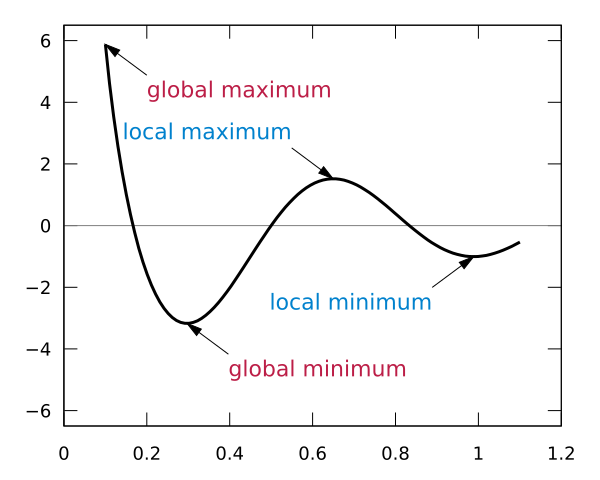
\includegraphics[scale=.5]{MATH_1060_Section_4-1_Extrema.PNG}
\end{center}

\boxenv{Definition.}{The maximum and minimum values of $f$ are collectively referred to as the \textbf{extreme values} or the \textbf{extrema} of $f$.}

\begin{center}
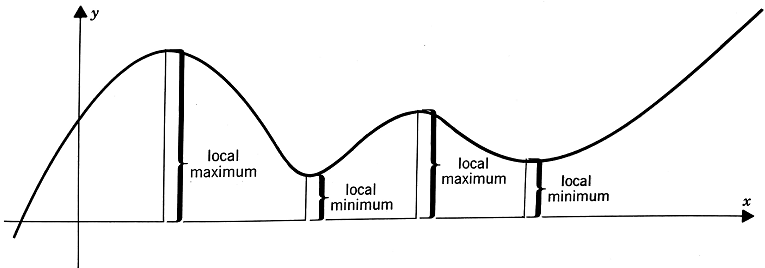
\includegraphics[scale=.7]{MATH_1060_Section_4-1_Maxima.PNG}
\end{center}

\boxenv{Definition.}{The number $f(c)$ is called a \textbf{local maximum} if it is the largest $y$-value in a ``window'' around $x=c$. 

\vspace{2mm}

The number $f(c)$ is called a \textbf{local minimum} if it is the smallest $y$-value in a ``window'' around $x=c$.}

\vspace{5mm}

By definition, local extrema may not occur at an endpoint. Note that some definitions use the word ``relative'' instead of ``local.''

\vspace{5mm}

\boxenv{Definition.}{The number $f(c)$ is called a \textbf{global maximum} if it is greater than or equal to all other $y$-values.

\vspace{2mm}

The number $f(c)$ is called a \textbf{global minimum} if it is less than or equal to all other $y$-values.}

\vspace{5mm}

It is possible for global extrema to occur at an endpoint. Some definitions use the word ``absolute'' instead of ``global.''

\vspace{3mm}

\Example Classify each of the extrema in the graph below as a local or global maximum or minimum.

\begin{center}
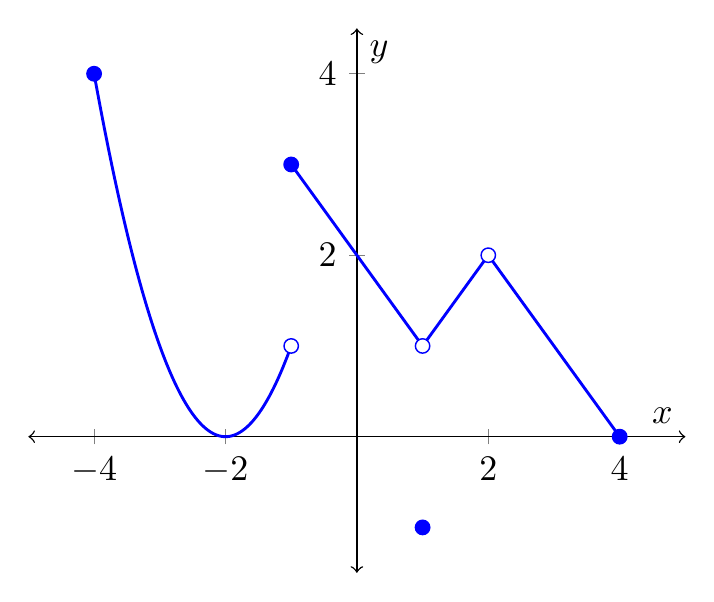
\begin{tikzpicture}[scale=1.3]
\begin{axis}[width=8cm,
	axis x line=middle,
	xmax=5, xmin=-5,
	axis y line=center,
	ymax=4.5, ymin=-1.5,
	axis line style=<->,
	xlabel=$x$,ylabel=$y$
    ]

    \addplot[name path=f,smooth,domain=-4:-1,color=blue,samples=100,thick] {(x+2)^2};	
    \addplot[name path=f,smooth,domain=-1:1,color=blue,samples=100,thick] {-x+2};
    \addplot[name path=f,smooth,domain=1:2,color=blue,samples=100,thick] {x};	
    \addplot[name path=f,smooth,domain=2:4,color=blue,samples=100,thick] {4-x};	
	
    \addplot[mark=*,color=blue] coordinates {(-4,4)};
    \addplot[mark=*,color=blue] coordinates {(-1,3)};
    %\addplot[mark=*,color=blue] coordinates {(2,3)};
    \addplot[mark=*,color=blue] coordinates {(1,-1)};
    \addplot[mark=*,color=blue] coordinates {(4,0)};
		    \addplot[mark=*,color=blue,fill=white] coordinates {(-1,1)};	
		    \addplot[mark=*,color=blue,fill=white] coordinates {(2,2)};	
		    %\addplot[mark=*,color=blue,fill=white] coordinates {(4,0)};	
		    \addplot[mark=*,color=blue,fill=white] coordinates {(1,1)};
	
						
\end{axis}
\end{tikzpicture}
\end{center}

\subsection*{Locating Extrema}

How can we locate extrema using tools we know without seeing the graph of the function?

\vspace{60mm}

\boxenv{Theorem.}{Suppose $f$ attains a maximal or minimal values at $x=c$. Then it must be that either $f'(c)=0$ or $f'(c)$ fails to exist.}

\vspace{5mm}

Note that the converse is \textbf{not} true: The fact that $f'(c)=0$ or $f'(c)$ fails to exist does not automatically imply the existence of a maximum or minimum. For example, consider the graph of $y=\lp x-\frac{1}{2}\rp^3+1$.

\begin{center}
\begin{tikzpicture}[scale=1.3]
\begin{axis}[width=8cm,
	axis x line=middle,
	xmax=2.5, xmin=-2.5,
	axis y line=center,
	ymax=4.5, ymin=-4.5,
	xlabel=$x$,ylabel=$y$,
	axis line style=<->
    ]

{
    \addplot[name path=f,smooth,domain=-1.2:1.9,color=blue,samples=200,thick,<->] {(x-0.5)^3+1};
    \addplot[mark=*,color=red] coordinates {(0.5,1)};

	}			
\end{axis}
\end{tikzpicture}
\end{center}

\vspace{1mm}

\paragraph{Critical Points.} Critical points are values that give \textit{candidates} for extrema. They allow us to determine (1) if we have a maximum or minimum and (2) if so, what type of maximum or minimum (i.e.\ global or local).

\vspace{3mm}

\boxenv{Definition.}{An \textit{interior point} $c\in\text{Dom}\ls f\rs$ is called a \textbf{critical point} if either $f'(c)=0$ or $f'(c)$ fails to exist.}

\newpage

First, we will focus on finding global extrema within a closed interval.

\vspace{5mm}

\boxenv{Extreme Value Theorem (EVT).}{Suppose $f$ is continuous on the closed interval $\ls a,b \rs$. Then there exists a minimum and maximum $y$-value on the interval.}

\vspace{50mm}

\paragraph{Applying the EVT.} If $f$ is continuous on $\ls a,b \rs$, then\dots
\begin{enumerate}
	\item[\tc{1}] Calculate $f(a)$ and $f(b)$.
	\item[\tc{2}] Find the critical points of $f$ on $\ls a,b \rs$, say $x=c_1$ and $x=c_2$. 
	\item[\tc{3}] Evaluate $f$ at the critical points, for example $f(c_1)$ and $f(c_2)$.
	\item[\tc{4}] The \textbf{global max} is the \textit{largest} of these values and the \textbf{global min} is the \textit{smallest} of these values.
\end{enumerate}

\vspace{3mm}

\Example Determine the global extrema of $g(x)=\disp\frac{4x}{x^2+1}$ on $\ls 0,2\rs$. 

\newpage

\Example Determine the global extrema of $f(x)=\ln(x^2+2)$ on $\ls -1,2\rs$.


\end{document}